\documentclass[border=6pt]{standalone}
\usepackage{amsmath}
\usepackage{tikz}
\usepackage{pgfplots}
\pgfplotsset{compat=1.18}
\usetikzlibrary{arrows.meta,calc,positioning}
\begin{document}
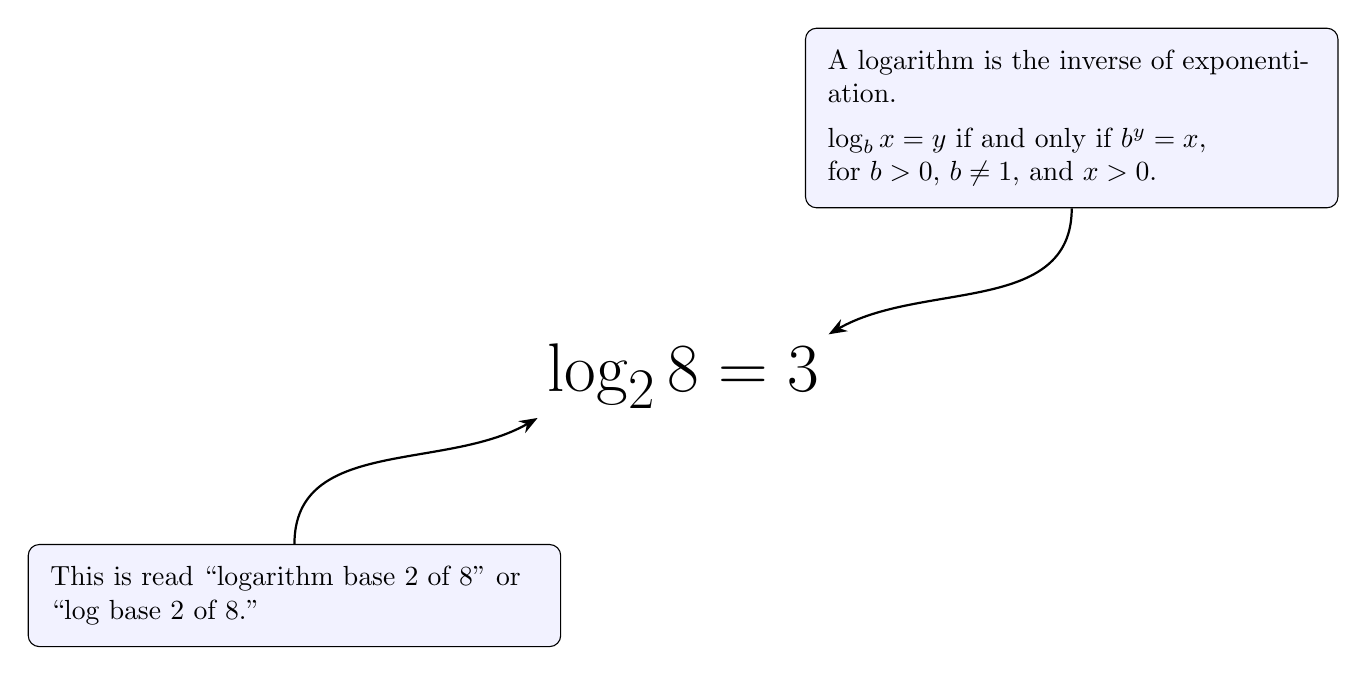
\begin{tikzpicture}[
    callout/.style={draw, rounded corners, fill=blue!5, align=left, text width=6.2cm, inner sep=8pt},
    >=Stealth,
]

% Central expression
\node[font=\Huge] (expr) at (0,0) {$\log_2 8 = 3$};

% First callout: reading the expression
\node[callout, below left=1.6cm and -0.3cm of expr] (read) {
  This is read ``logarithm base 2 of 8'' or ``log base 2 of 8.''
};
\draw[->, thick] (read.north) to[out=90,in=210] (expr.south west);

% Second callout: definition of a logarithm
\node[callout, above right=1.6cm and -0.3cm of expr] (def) {
  A logarithm is the inverse of exponentiation.\\[4pt]
  $\log_b x = y$ if and only if $b^y = x$,\\
  for $b>0$, $b\ne 1$, and $x>0$.
};
\draw[->, thick] (def.south) to[out=270,in=30] (expr.north east);

\end{tikzpicture}
\end{document}
